\chapter{Event generation, simulation and reconstruction \label{chap:event_generation}}

\section{What is an ``event''? \label{sec:event}}

% add picture of CMS event display
% add picture of hadronization etc for event

\section{Event generation \label{sec:event_generation}}

% add info on Madgraph, pythia, jet matching etc

\section{Event simulation \label{sec:event_simulation}}

\subsection{CMS Full Simulation using Geant4 \label{subsec:fullsim}}

% add some info on how this is done, particle interaction with matter, ionization, 
% how it deals with long lived particles?

\subsection{CMS Fast Simulation \label{subsec:fastsim}}

% explain what approximations are made, why it is necessery, especially in SUSY searches

\section{Event reconstruction \label{sec:event_reconstruction}}

% Add subsection on each object with all the object definitions we use

We select events with at least one interaction vertex, associated with at least 4 charged-particle
tracks, that lies within 24~cm of the origin of the CMS coordinate system along the beam direction
and 2~cm from the origin in the plane transverse to the beam. Owing to the high luminosity of the
LHC, hard scattering events are typically accompanied by many additional events arising from the
multiple proton-proton interactions that occur when the proton bunches cross.  The overlapping of
events is referred to as pileup.  The primary vertex is identified as the vertex with the highest
value of the $\sum \pt^2$ of the associated tracks.  Detector- and beam-related cleaning algorithms
are used to remove events with detector noise that mimic events with high energy and large imbalance
in transverse momentum.  


 \subsection{Event Cleaning \label{sec:event_cleaning}}
% 
% We follow the recommended procedure set out by the JetMET POG, and apply a series of event filters.
% These are:
% 
% \begin{itemize}
% \item The {\tt EcalDeadCellTriggerPrimitiveFilter}, which removes events where dead cells in the
% ECAL produce anomalous activity.
% \item The {\tt hcalLaserEventFilter}, which removes events where the HCAL laser produces anomalous
% activity.
% \item The {\tt hcalLaserEventFilter2012}, 
% \item The {\tt trackingFailureFilter}, which removes events where the tracking algorithm does not
% perform properly.
% \item The {\tt CSCTightHaloFilter}, which removes events contaminated by beam halo.
% \item The {\tt HBHENoiseFilter}, which removes events featuring large hadronic calorimeter noise.
% \item The {\tt eeBadScFilter}, which removes events featuring high amplitude anomalous pulses due to
% bad ECAL super-crystals.
% \item The {\tt trkPOGFilters}, which remove events due to track reconstruction anomalies, such as
% events with partly aborted track reconstruction and events affected by the Strip Tracker coherent
% noise.
% \item The {\tt primaryVertexFilter}, which removes events that do not have a good primary vertex.
% \item The {\tt noscrapingFilter}, which removes events with a large multiplicity of low quality
% tracks.
% \end{itemize}
% 
% More details on these filters can be found in Ref.~\cite{metfilters}. For MC samples that are passed
% through the fast CMS detector simulation, the {\tt CSCTightHaloFilter} and {\tt HBHENoiseFilter}
% filters are not applied, as their input collections are not produced in {\sc FastSim} productions.
% 
% In addition to the filters listed above, we also use a cleaning cut to remove events with spurious
% HCAL noise. This is explained in more detail in section~\ref{sec:noise}. 


\subsection{Particle Flow technique \label{sec:event_reco_pf}}

CMS reconstructs events using the particle flow (PF) method~\cite{PF}, which reconstructs particles
(PF candidates) by combining information from the inner tracker, the calorimeters, and the muon
system.  Each PF candidate is a ssigned to one of five object categories: muons, electrons, photons,
charged hadrons, and neutral hadrons.  Contamination from pileup events is reduced by discarding
charged PF candidates that are incompatible with having originated from the primary
vertex~\cite{CMS-PAS-JME-14-001}.   The average pileup energy due to neutral hadrons is computed
event-by-event and subtracted from the energy when computing lepton isolation and jet energy.  The
energy subtracted is  the average pileup energy per unit area (in $\Delta\eta \times \Delta\phi$)
times the jet area~\cite{Fastjet1, Fastjet2}.

\subsection{Object identification}

Jets are clustered with \textsc{FastJet 3.0.1}~\cite{Cacciari:2011ma} using the anti-$k_\textrm{T}$
algorithm~\cite{antikt} with size parameter $\Delta R=0.5$ (AK5).  Jet corrections are applied as a
function of jet $\pt$ and $\eta$ to account for the residual effects of non-uniform detector
response.  
The  jet energies are corrected so that, on average, they match those of simulated particle-level
jets. After correction, jets are required to have $\pt > 30$~\GeV and $|\eta| < 2.4$.  We use the
combined secondary vertex algorithm~\cite{btag7TeV,btag8TeV} to identify jets arising from $\cPqb$
quarks. The medium tagging condition, which yields a $\cPqb$  jet misidentification rate of
$\sim$1\% and a typical efficiency of $\sim$70\%, is used to select $\cPqb$ jets. The loose tagging
condition, with a misidentification rate of $\sim$10\% and efficiency of $\sim$85\%, is used to veto
$\cPqb$ jets.  

Missing transverse energy, which is used in the calculation of the razor variable $\mr$, is 
defined to be the negative sum of the transverse momenta of all the particle flow objects in an
event.  Loosely identified and isolated electrons with $\pt > 5$~\GeV and $|\eta| < 2.5$ and muons
with $\pt > 5$\GeV and $|\eta| < 2.4$ are used both to suppress backgrounds in our signal region and
in the definition of the control regions.  A tight definition of isolated leptons (electrons with
$\pt > 10$~\GeV and $|\eta| < 2.5$ and muons with $\pt > 10$~\GeV and $|\eta| < 2.4$) defines a
control region enriched in $\cPZ \rightarrow \ell \ell $ events, from which we estimate the
systematic uncertainty in the predicted number of $\cPZ \rightarrow \nu \nu$ events in the signal
region. Any electron candidates with $1.44 < |\eta| < 1.57$ are rejected since the transition region
between barrel and endcap calorimeters is less well-instrumented.
In order to suppress the decays of taus and other leptons that fail the loose selection, events that
have isolated tracks with $\pt > 10$\GeV and track-primary vertex distance along the beam direction
$dz < 0.05$ are rejected.

\subsubsection{Jets \label{sec:object_jets}}



%%%%%%%%%%%%%%%%%%%%%%%%%%%%%%%%%%%%%%%%%%%%%%%%%%%%%%%%%%%%%%%%%%%%%%%%%%%%%%%%%%%%%%%%%%%%%%%%%

% \subsection{Vertex Selection \label{sec:vertex}}
% 
% We require at least one {\it good} vertex to be reconstructed in each event, according to the
% definitions given in Table~\ref{tab:vertex}.
% 
% \begin{table}[htdp]
% \caption{Vertex selection \label{tab:vertex}}
% \begin{center}
% \begin{tabular}{|ll|}
% \hline
% \multicolumn{2}{|l|}{CMSSW collection label: goodOfflinePrimaryVertices} \\
% \multicolumn{2}{|l|}{CMSSW type: reco::Vertex} \\
% \hline
% Variable/Method & Value \\
% \hline
% isFake() & $= 0$ \\
% ndof() & $> 4$ \\
% z() & $< 24$ \\
% position.Rho() & $< 2$ \\
% \hline
% \end{tabular}
% \end{center}
% \end{table}
% 
% The highest sum-$p_T$ vertex is chosen as the reference primary vertex in the event. This vertex is
% taken as a reference to reconstruct the event, e.g. to perform the track subtraction for pileup
% removal, for which we use the {\tt PFNoPileUp} algorithm.


% \subsection{Jet Reconstruction \label{sec:jets}}
% 
% We consider the list of reconstructed particle-flow jets, clustered with the {\it anti-$k_t$}
% algorithm and cone-size parameter $\Delta R=0.5$.  The jets are corrected for pile-up effects in a
% two step process.  First charged hadron particle-flow candidates that have been associated with a
% pile-up vertex are removed from the list of particles to be clustered using the {\tt PFNoPileUp}
% algorithm.  The jets are then clustered and corrected for the L2 and L3 corrections, taking into
% account the charged-hadron removal. The remaining PU energy is subtracted by applying the
% event-by-event quantity $\pi \rho (\Delta R)^2$, where $\Delta R$
% is the jet size and $\rho$ is the average density from PU events, as computed by {\tt FastJet} using
% only neutral hadron particle-flow
% candidates.  This procedure is the one recommended by the JetMET POG and is implemented using
% standard CMSSW tools. Our jet selection is defined in Table~\ref{tab:jets}.  
% 
% The AK5 jets defined above are used for most of the analysis (including the construction of the
% megajets for the calculation of the razor variables), except when reconstructing hadronic
% $W$-candidates and applying jet substructure cuts. 
% To do this, jets are clustered using the Cambridge-Aachen algorithm, with distance parameter
% $R=0.8$. More details on this can be found in section~\ref{sec:Wtagging}.
% 
% \begin{table}[htdp]
% \caption{Jet selection \label{tab:jets}}
% \begin{center}
% \begin{tabular}{|ll|}
% \hline
% \multicolumn{2}{|l|}{CMSSW collection label: } \\
% \multicolumn{2}{|l|}{CMSSW type: pat::Jet} \\
% \hline
% Variable/Method & Value \\
% \hline
% pt() & $> 30$ \\
% eta() & $< 2.4$ \\
% neutralHadronEnergyFraction() & $< 0.99$ \\
% neutralEmEnergyFraction() & $< 0.99$ \\
% nConstituents() & $> 1$ \\
% chargedHadronEnergyFraction() & $> 0$ \\
% chargedMultiplicity() & $> 0$ \\
% chargedEmEnergyFraction() & $< 0.99$ \\
% \hline
% \end{tabular}
% \end{center}
% \end{table}



% \subsection{B-Tagging \label{sec:btag}}
% 
% As the signal in this analysis is enriched in $b$-quarks, we use the combined secondary vertex (CSV)
% algorithm to identify jets that are consistent with coming from $b$ decays. We use the recommended
% loose and medium working points from the BTag POG, shown on Table~\ref{tab:btag} with no further
% cuts on the jets \cite{BTagWP}. The loose working point is used as a veto to identify $t\bar{t}$
% (and signal) depleted control regions, while the medium working point is used to define signal
% enriched regions in which to perform the analysis.
% 
% \begin{table}[htdp]
% \caption{b tagging definition \label{tab:btag}}
% \begin{center}
% \begin{tabular}{|lll|}
% \hline
% \multicolumn{3}{|l|}{CMSSW collection label: } \\
% \multicolumn{3}{|l|}{CMSSW type: pat::Jet} \\
% \hline
% Working point & Variable/Method & Value \\
% \hline
% CSV Medium & combinedSecondaryVertexBJetTags() & $> 0.679$ \\
% CSV Loose & combinedSecondaryVertexBJetTags() & $> 0.244$ \\
% \hline
% \end{tabular}
% \end{center}
% \end{table}
% 
% As will be explained in section~\ref{sec:selection}, we define our signal and control regions based
% on the number of b-tagged jets. 
% As the b-tagged jet multiplicity distribution is not exactly the same in data as in simulation, we
% need to apply appropriate Data/MC scale factors to the simulation. These scalefactors and their
% prescription have been provided by the BTag POG \cite{BTagSF1,BTagSF2}. 
% Whenever an explicit selection based on the number of b-tagged jets is made, the btag scale factors
% are applied to the simulation. 
% For more detailed information on the scale factors and their associated uncertainties, we refer to
% section~\ref{sec:btag_uncertainties}. 


% \subsection{Muon Selection \label{sec:muon}}
% 
% We identify muons at two different working points; a tight selection and a loose selection. 
% Currently we mainly use the loose definition in the analysis, both for vetoing, and for selecting
% single muon events for the control regions enriched in TTJets and WJets. The tight selection is only
% used to define a control region enriched in $Z\rightarrow ll$ events, from which we derive a
% systematic uncertainty on the predicted number of $Z\rightarrow\nu\nu$ events in our signal region.
% 
% \subsubsection{Tight selection \label{sec:tightmuon}}
% 
% The tight selection follows the tight-muon recommendation from the Muon POG \cite{MuonID}. A summary
% of the selection can be found in table~\ref{tab:tightmuon}. 
% We also require the muon to be isolated. This isolation is calculated
% using the particle-flow candidates after charged-hadron candidates
% associated from pile-up vertexes have been removed in a cone of size 0.4. The removed
% charged hadrons are used to estimate the remaining contribution to the
% isolation coming from neutral hadrons from pile-up. The isolation
% definition used is:
% \begin{equation}
% I_\mu(p_t^\mu) = \left[ I_{Charged} + I_{Neutral} + I_{\gamma} - (\Delta\beta\cdot
% I_{Charged}^{PU})\right] /p_T^\mu, ~~
% \label{eqn:iso}
% \end{equation}
% where $\Delta\beta$ is 0.5 and $I_\mu$ is required to be less than 0.15.
% 
% 
% \begin{table}[htdp]
% \caption{Tight muon definition}
% \begin{center}
% \begin{tabular}{|ll|}
% \hline
% \multicolumn{2}{|l|}{CMSSW collection label: } \\
% \multicolumn{2}{|l|}{CMSSW type: pat::Muon} \\
% \hline
% Variable/Method & Value \\
% \hline
% pt() & $> 10$ \\
% fabs(eta()) & $< 2.4$ \\
% isPFMuon() & $= 1$ \\
% isGlobalMuon() & $= 1$ \\
% globalTrack().normalizedChi2() & $< 10$ \\
% globalTrack().hitPattern().numberOfValidMuonHits() & $> 0$ \\
% track().hitPattern().trackerLayersWithMeasurement() & $> 5$ \\
% innerTrack().hitPattern().numberOfValidPixelHits() & $> 0$ \\
% numberOfMatchedStations() & $> 1$ \\
% fabs(innerTrack().dxy(vertex.position())) & $< 0.2$ \\
% fabs(muonBestTrack().dz(vertex.position())) & $< 0.5$ \\
% \hline
% relIso $=$ (pfIsolationR04().sumChargedHadronPt() $+$ & \\
% \hspace{1.3cm} max(0., pfIsolationR04().sumNeutralHadronPt() $+$ & \\
% \hspace{1.3cm} pfIsolationR04().sumPhotonPt() $-$ & \\
% \hspace{1.3cm} 0.5pfIsolationR04().sumPUPt()))/pt() & $< 0.15$ \\ 
% \hline
% \end{tabular}
% \end{center}
% \label{tab:tightmuon}
% \end{table}
% 
% \subsubsection{Loose selection \label{sec:loosemuon}}
% 
% We take the loose muon selection from stop working group recommendations \cite{StopWG}. The exact
% details and performance of this selection is documented in Ref.~\cite{Ra2Top}. The main difference
% between this selection and the muon POG selections is that a {\em directional} isolation is used
% that has been optimised for events with much hadronic activity. This is defined as below, and is
% particularly useful for rejecting events with leptons coming from $b$-quark decays.
% \[
% \overrightarrow{\mathrm{ISO}}_{R}\equiv\sum_{\Delta R_{i}<R}\delta_{i}^{2}\pt{}_{i}
% \]
% where the sum is over all other particles $i$ within $\Delta R<R$ of the lepton direction, and
% $\delta_{i}$ is the angle between particle $i$ and the $\pt$-weighted centroid position
% ($\delta_{c}$) of all such particles in $\eta-\phi$ space. That is, if $\Delta\phi_i$ and
% $\Delta\eta_i$ are respectively the difference in $\phi$ and $\eta$ angles between particle $i$ and
% the lepton, then:
% \begin{eqnarray*}
% \vec{e}_{i} & \equiv & \frac{1}{\sqrt{\Delta\phi_{i}^{2}+\Delta\eta_{i}^{2}}}\left(\begin{array}{c}
% \Delta\phi_{i};\\
% \Delta\eta_{i}
% \end{array}\right);\\
% \vec{\delta}_{c} & = & \sum_{\Delta R_{i}<R}\pt{}_{i}\vec{e}_{i};\\
% \delta_{i} & = &
% \angle(\vec{\delta}_{c},\vec{e}_{i})=\arccos(\vec{\delta}_{c}\cdot\vec{e}_{i}/|\vec{\delta}_{c}|).
% \end{eqnarray*}
% $\vec{e}_{i}$ is the unit vector specifying particle $i$'s relative location in $\eta-\phi$ space.
% 
% Loose Muons are reconstructed using either the global or tracker-only algorithms. 
% Global-reconstructed muons are required to pass the {\tt GlobalMuonPromptTight} quality criteria,
% plus to have at least two muon chambers containing segments uniquely matched to its inner track. 
% Tracker-only muons are required to pass the {\tt TMLastStationTight} criteria, which requires the
% muon to have  compatible hits in the last muon chamber. All selected muons are then required to pass
% cuts in the following variables:
% \begin{itemize}
% \item $p_T > 5$GeV;
% \item $|\eta| < 2.4$; 
% \item At most 1 lost [expected] inner tracker hits for $\pt < 20\GeV$ muons.
% \item At most 4 lost [expected] inner tracker hits for $\pt \geq 20\GeV$ muons.
% \item $\pt$- and $\eta$-dependent maximum $d_{xy}$, the impact parameter of the inner track w.r.t.
% the primary vertex.
% \item $\pt$- and $\eta$-dependent maximum $d_{z}$, the absolute difference between the muon and
% primary vertex $z$-positions.
% \item $\pt$- and $\eta$-dependent maximum directional isolation sum with $R = 0.2$.
% \end{itemize}
% The details of the $\pt$- and $\eta$ dependent cuts can be found in Ref.~\cite{Ra2Top}.

% \subsection{Electron selection \label{sec:electron}}
% 
% We identify electrons at two different working points; a tight selection and a loose selection. 
% Currently we mainly use the loose definition in the analysis, both for vetoing, and for selecting
% single electron events for the control regions enriched in TTJets and WJets. The tight selection is
% only used to define a control region enriched in $Z\rightarrow ll$ events, from which we derive a
% systematic uncertainty on the predicted number of $Z\rightarrow\nu\nu$ events in our signal region.
% 
% \subsubsection{Tight Selection \label{sec:tightele}}
% 
% \begin{table}[htdp]
% \caption{Tight electron definition}
% \begin{center}
% \begin{tabular}{|lll|}
% \hline
% \multicolumn{3}{|l|}{CMSSW collection label: } \\
% \multicolumn{3}{|l|}{CMSSW type: pat::Electron} \\
% \hline
% Variable/Method & \multicolumn{2}{l|}{Value} \\
% \hline
% pt() & $> 10$ & \\
% fabs(eta()) &  \multicolumn{2}{l|}{$< 2.5$ and not in $1.442 - 1.556 $} \\
% \hline
% ID & Barrel & Endcap \\
%      & $|\eta| < 1.479$ & $1.479 < |\eta| < 2.5$ \\
%      & isEB() $= 1$ & isEE() $= 1$ \\ 
% \hline
% deltaEtaSuperClusterTrackAtVtx() & $< 0.004$ & $< 0.007$ \\
% deltaPhiSuperClusterTrackAtVtx() & $< 0.060$ & $< 0.030$ \\
% sigmaIetaIeta() & $< 0.010$ & $< 0.030$ \\
% hadronicOverEm() & $< 0.120$ & $< 0.100$ \\
% 1.0/ecalEnergy() - eSuperClusterOverP()/ecalEnergy() ) & $< 0.050$ & $< 0.050$ \\
% gsfTrack().get().trackerExpectedHitsInner().numberOfHits() & $\le 1$ & $\le 1$ \\
% passConversionVeto() & $= 1$ & $= 1$ \\
% \hline
% \end{tabular}
% \end{center}
% \label{tab:tightele}
% \end{table}
% 
% 
% 
% The tight electron selection is taken from the EGamma POG \cite{ElectronID}. A summary of the
% selection can be found in table~\ref{tab:tightele}. 
% 
% We also require to electron to be isolated. The isolation is calculated using the particle-flow
% candidates in a cone of size 0.3 around the electron, and then corrected with an estimate of the
% median energy from pile-up as calculated with the {\tt FastJet} algorithm in a similar way to the
% jet corrections explained in Sec.~\ref{sec:jets}. We require that this corrected isolation, weighted
% by the $p_T$ of the electron is less than 0.15.
% 
% \begin{equation}
% I_e(p_T^e) = \left[ I_{Charged} + \max(0., (I_{NeutralHad} + I_{\gamma})) - A \rho \right] / p_T^e
% \qquad
% \end{equation}
% 
% \subsubsection{Loose electron selection \label{sec:looseele}}
% 
% As for the muons, we follow the stop working-group's recommendation for a loose-electron
% identification \cite{StopWG}. The exact details and performance of this selection is documented in
% Ref.~\cite{Ra2Top}. In summary, we require:
% \begin{itemize}
% \item $p_T > 5 \GeV$;
% \item $|\eta| < 2.5$ and ($|\eta| < 1.442$ OR $|\eta| > 1.556$) ; 
% \item No lost [expected] tracker hits for $\pt < 20\GeV$ electrons.
% \item At least 2 (1) pixel hits for $\pt < 10\GeV$ electrons in the barrel (endcap). 
% \item $\pt$- and $\eta$-dependent maximum $d_{z}$, the absolute difference between the electron and
% primary vertex $z$-positions.  
% \item $\pt$- and $\eta$-dependent maximum directional isolation sum with $R = 0.3$ and calculated
% with only charged particles.
% \item For electrons in the barrel only: an additional $\pt$- and $\eta$-dependent maximum
% directional isolation sum with $R = 0.2$ and calculated using all particles.
% \end{itemize}
% Details of the $\pt$- and $\eta$-dependent cuts can be found in Ref.~\cite{Ra2Top}, and a
% description of the directional isolation can be found in Sec.~\ref{sec:loosemuon}.
% 
% 
% \subsection{Isolated tracks \label{sec:isolatedtrack}}
% 
% In order to suppress the decays of both taus and other leptons that do not pass the loose selection,
% we employ an isolated track veto at particle-flow candidate level, following
% Ref.~\cite{StopSingleLepton}.  
% Isolated tracks are selected from the charged particle flow candidates with $p_T > 10\GeV$ and
% longitudional track-primary vertex distance of $dz < 0.05$.  
% 
% In the hadronic event selection, events with an isolated track will be vetoed.  
% 
% In event selections involving a tight lepton (none existent in the analysis at this point), isolated
% track veto can be used for vetoing events with a second lepton.  In this case, in order to ensure
% that the track under question does not belong to the tight lepton, $dR(\ell_{tight}, track) > 0.3$
% is required.  
% 
% \begin{table}[htdp]
% \caption{Isolated track selection.  See Section~\ref{sec:vertex} for primary vertex definition and
% Sections~\ref{sec:tightmuon} and~\ref{sec:tightele} for tight muon and electron definitions.}
% \begin{center}
% \begin{tabular}{|ll|}
% \hline
% \multicolumn{2}{|l|}{CMSSW collection label: pfNoPileUp} \\
% \multicolumn{2}{|l|}{CMSSW type: reco::PFCandidate} \\
% \hline
% Variable/Method & Value \\
% \hline
% pt() & $= 0$ \\
% charge() & $> 0$ \\
% $dz($PV, track$)$ & $< 0.05$ \\
% $\left[ \sum_{j \neq i} pt()_j \right] / pt()_i$ & $< 0.1$ \\
% \hline
% \multicolumn{2}{|l|}{For selections with tight leptons:} \\
% \hline
% $dR(\ell_{tight}, {\rm track})$ & $ > 0.3$ \\
% \hline
% \end{tabular}
% \end{center}
% \label{tab:isolatedtrack}
% \end{table}
% 
% We remove particle-flow candidates corresponding to an electron or muon passing the tight selection
% with a $\Delta R$ cut of 0.1. Isolated tracks are those particle-flow candidates coming from the
% primary vertex that are charged, have $p_T > 10$GeV and have relative isolation in a cone of size
% 0.3 less than 0.1. In the leptonic final states, the isolated track veto is only applied if the
% charge of the track is opposite to that of the tight lepton.


% \subsection{Missing Energy}\label{sec:met}
% 
% We use the particle-flow candidates to calculate the transverse missing energy (MET) of the event.
% As recommended by the JetMET POG, we apply appropriate jet-energy scale corrections (type-1 only).
% No explicit selection is made on the missing-energy, however, it is correlated with the razor
% variable $M_R^T$, introduced in section~\ref{sec:razor}.
% 
% \subsection{HCAL Noise}\label{sec:noise}
% 
% Starting with the 52X releases of CMSSW, the reconstruction of particle-flow jets and particle-flow
% MET  
% includes energy measured in the CMS Hadron Outer Calorimeter (HO), while the reconstruction of 
% calorimetric jets and calorimetric MET does not. 
% 
% Events may receive a large, anomalous contribution to the PF MET from HO energy. 
% In these events, the PF MET differs from the calo MET substantially, 
% even in the absence of muons (which also contribute to the PF MET but not the calo MET).
% Since no filter has yet been developed,
% we implement a cleaning cut to remove these events. In the following PF MET 
% always refers to type-1 corrected PF MET, while CALO MET refers to the global muon corrected calo
% MET.
% 
% We cut events in which the PF MET vector $\MET^{,\textrm{PF}}$ is flipped with respect 
% to the calo MET vector $\MET^{,\textrm{CALO}}$. 
% To accomplish this we compute the absolute value of the difference in polar angle
%  $|\Delta\phi_{\textrm{PF,CALO}}|$, taken to in the range $[0,2\pi)$, and defined as
% \begin{equation}
%  \phi^{\textrm{PF}} = \textrm{arctan}\left( \frac{\MET^{,\textrm{PF}}_y}{\MET^{,\textrm{PF}}_x}
% \right) ,~~~~
%  \phi^{\textrm{CALO}} = \textrm{arctan}\left(
% \frac{\MET^{,\textrm{CALO}}_y}{\MET^{,\textrm{CALO}}_x} \right)
% \end{equation}
% \begin{equation}
% |\Delta\phi_{\textrm{PF,CALO}}| = \min \left ( \phi^{\textrm{PF}} - \phi^{\textrm{CALO}},   2\pi -
% \phi^{\textrm{PF}} + \phi^{\textrm{CALO}} \right)
% \end{equation}
% 
% Then we cut events in which $|\Delta\phi_{\textrm{PF,CALO}}|$ falls in a 1 radian ($\sim57$ degree)
% window centred around $\pi$. This cut is applied to all boxes to remove anomalous events with large
% PF MET.
% \begin{equation}
% ||\Delta\phi_{\textrm{PF,CALO}}| -\pi | < 1
% \label{eqn:dphicut}
% \end{equation}

% \subsection{Pileup reweighting \label{sec:pileup}}
% 
% The distribution of the number of pileup interactions is different in Data vs MC. 
% As the number of pileup interactions can have an influence on various aspects of the reconstruction,
% we need to reweight the MC events to match the pileup distribution in data. 
% The method to do this is quite straightforward. 
% 
% \begin{enumerate}
% 
% \item Determine the pileup distribution in data by using a centrally provided script:
% {\footnotesize
% \begin{verbatim}
% pileupCalc.py -i Cert_190456-208686_8TeV_22Jan2013ReReco_Collisions12_JSON.txt 
%               -o data_pileup.root --inputLumiJSON=pileup_latest.txt 
%               --calcMode=true --minBiasXsec=69400 --maxPileupBin=100
% \end{verbatim}
% }
% In this, \texttt{pileup\_latest.txt} is taken directly from the central DQM area, as is the Lumi
% JSON. The Lumi JSON used is the one for the full Jan22 ReReco, corresponding to the data we are
% using, see section~\ref{sec:samples}. 
% 
% \item Determine the pileup distribution in simulation: \\ 
% For this we use a variable called \texttt{trueNumInteractions}. 
% The distribution of this variable for all MC events is used as the pileup distribution for Monte
% Carlo. 
% 
% \item Normalize the MC and data histograms to unit area, and divide them (Data/MC). The resulting
% histogram contains the event weights. 
% 
% \item Apply these event weights to each MC event, by picking up the value for
% \texttt{TrueNum\-Interactions} for that event, finding in what bin it falls and then applying the
% corresponding weight.
% 
% \end{enumerate}
% 
% The distribution of the pileup in data and simulation, and the corresponding pileup weight is shown
% in Figure~\ref{fig:DataMC_pileup} for the FullSim simulation and in figure~\ref{fig:DataMC_pileup52}
% for the FastSim simulation using CMSSW\_52X. 
% 
% \begin{figure}[p]
%  \centering
%  \includegraphics[width=0.7\textwidth]{figures/Pileup/compare_pileup_profile}
% \caption{Comparison plot of the true number of interactions in data and in MC. On the top the
% distribution of both are shown, on the bottom the ratio Data/MC. Left is linear scale, right is log
% scale. 
% \label{fig:DataMC_pileup}}
% \end{figure}
% 
% \begin{figure}[p]
%  \centering
%  \includegraphics[width=0.7\textwidth]{figures/Pileup/compare_pileup_profile_52X}
% \caption{Comparison plot of the true number of interactions in data and in MC processed with
% CMSSW\_52X. On the top the distribution of both are shown, on the bottom the ratio Data/MC. Left is
% linear scale, right is log scale. 
% \label{fig:DataMC_pileup52}}
% \end{figure}
% 
% As a test of the performance of the pileup reweighting, we can check the agreement between data and
% simulation for the distribution of the number of good primary vertices ($PV$) at different selection
% levels. 
% We expect to find a reasonable, although not perfect agreement as the vertex reconstruction
% efficiency depends on many things. 
% This comparison is shown in figure~\ref{fig:comparison_PV}. 
% 
% \begin{figure}
%  \includegraphics[width=0.49\textwidth]{figures/Pileup/DataMC_PV_0Lb1Ll}
%  \includegraphics[width=0.49\textwidth]{figures/Pileup/DataMC_PV_g1Mb1Ll}
% \caption{Data/MC comparison plot of the number of good primary vertices after pileup reweighting for
% a control region enhanced in $W+$jets (left) and enhanced in $t\bar{t}+$jets (right).
% \label{fig:comparison_PV}}
% \end{figure}


% \subsection[Top pt reweighting]{Top \pt reweighting \label{sec:toppt_reweighting}}
% 
% The TOP group has found in the normalized differential top-quark-pair cross section analysis that
% the shape of the \pt spectrum of the individual top quarks in data is softer than predicted by the
% various simulations while the available approx. NNLO prediction delivers a reasonable description.
% Based on this measurement, they have derived event scalefactors with associated systematic
% uncertainties to test the potential impact of the modelling of the top quark \pt spectrum
% \cite{TopPt}. 
% 
% The event weight is derived as a function of the generated \pt of both the top and anti-top quark in
% the event: 
% \begin{equation}
% w_{\textrm{TopPt}} = \sqrt{ SF_t * SF_{\bar{t}} }
% \end{equation}
% \begin{equation}
% SF(\pt^{gen}) = \exp(a + b \pt^{gen})
% \end{equation}
% with $a = 0.156$ and $b = -0.00137$.
% 
% The uncertainty on this reweighting is given by the following prescription: 
% \begin{align}
% +1~\sigma &: w = w_{\textrm{TopPt}} * w_{\textrm{TopPt}} \\
% -1~\sigma &: w = 1 
% \end{align}
% where $w$ is the weight to be applied to the event for the up/down variation. 
% 
% In figure~\ref{fig:TopPt} we show the Data/MC comparison for the $M_R$ and $R^2$ distribution in the
% $t\bar{t}+$jets control region (see section~\ref{sec:Tregion}) before and after applying the
% reweighting procedure. 
% We observe that this reweighting greatly improves the agreement between data and simulation. 
% Therefore we will always apply this reweighting to the $t\bar{t}+$jets simulated sample. 
% 
% \begin{figure}[htpb]
% \centering
% \includegraphics[width=0.49\textwidth]{
% figures/DataMC/DataMC_MR_g1Mbg1W1LlmT100_mdPhig0p5_width_noTopPt}
% \includegraphics[width=0.49\textwidth]{
% figures/DataMC/DataMC_R2_g1Mbg1W1LlmT100_mdPhig0p5_width_noTopPt}
% 
% 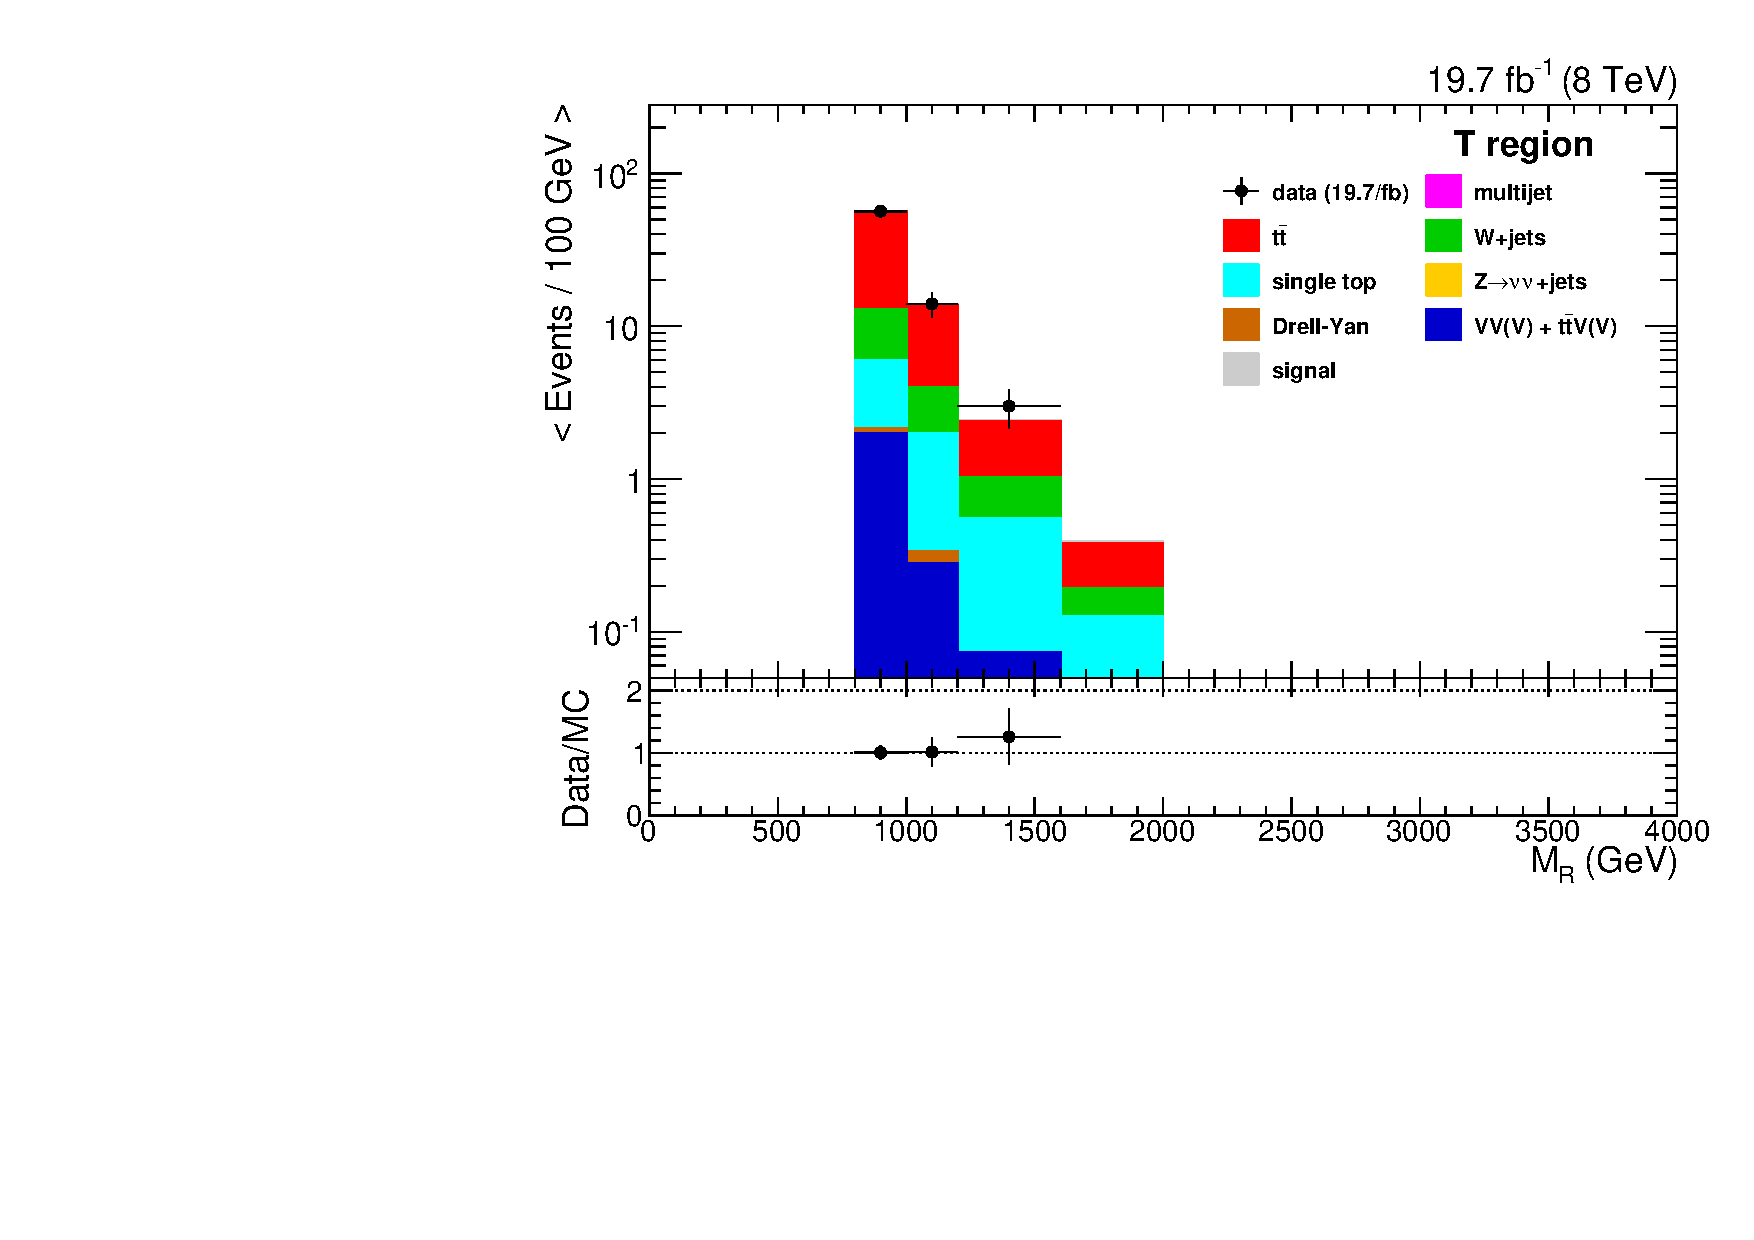
\includegraphics[width=0.49\textwidth]{figures/DataMC/DataMC_MR_g1Mbg1W1LlmT100_mdPhig0p5_width}
% 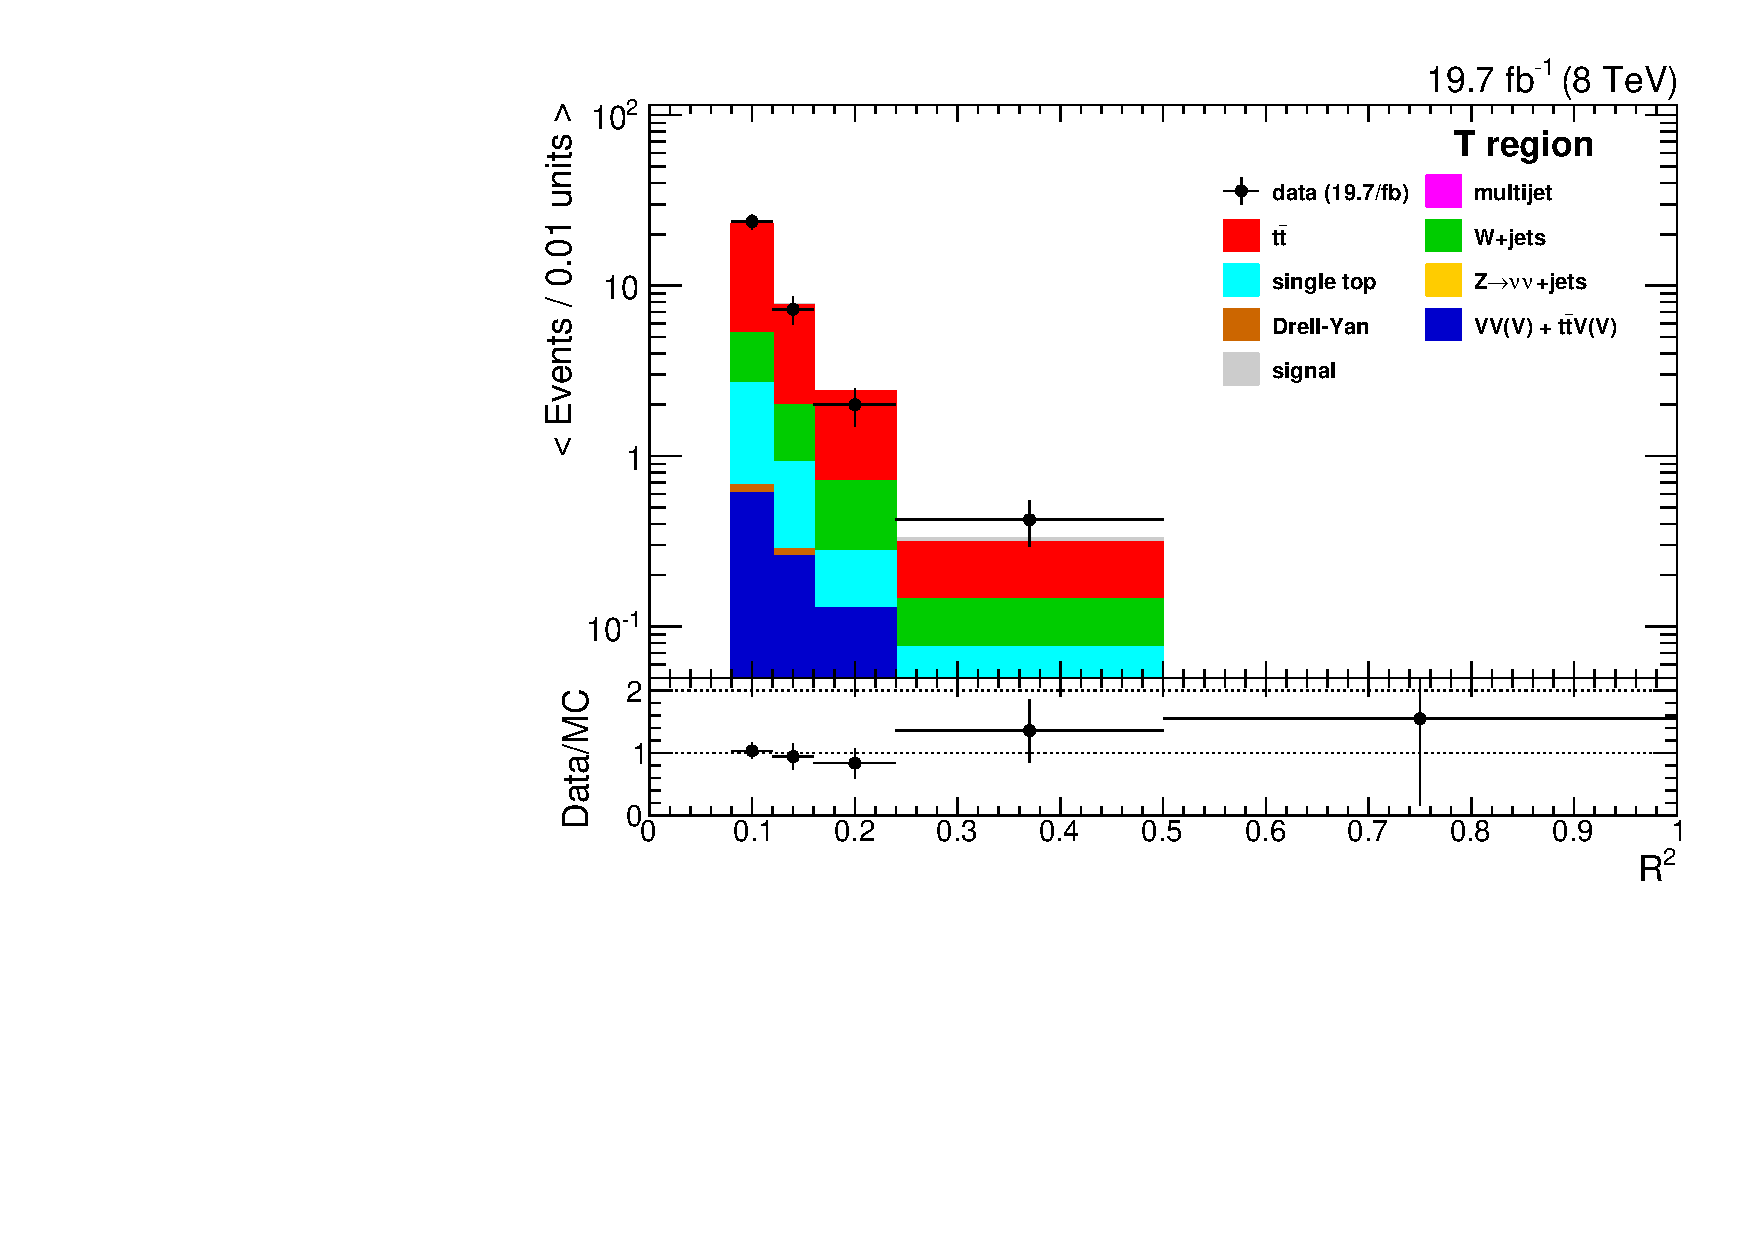
\includegraphics[width=0.49\textwidth]{figures/DataMC/DataMC_R2_g1Mbg1W1LlmT100_mdPhig0p5_width}
% \caption{[top] $M_R$ (left) and $R^2$ (right) distribution before applying the top \pt reweighting
%          [bottom] $M_R$ (left) and $R^2$ (right) distribution after applying the top \pt reweighting
% for the $T$ region as defined in section~\ref{sec:Tregion}
% \label{fig:TopPt}}
% \end{figure}

% 
% \subsection{ISR reweighting \label{sec:ISRreweighting}}
% 
% As recommended, we apply the ISR reweighting recipe developed in the SUSY group
% \cite{ISRreweighting} to all our simulated signal samples.
% Each event is reweighted with an event weight, depending on the \pt of the system that is recoiling
% against the ISR jet(s). 
% For the T1ttcc simplified model this system is the system of the two gluinos. For T2tt this is the
% system of the two stop squarks. 
% In table~\ref{tab:ISRreweighting} we list the scale factor to be applied for the different \pt
% ranges. 
% The difference between that scale factor and 1 is taken to be the one standard deviation
% uncertainty. 
% 
% \begin{table}[htpb]
% \centering
% \caption{ISR reweighting prescription \label{tab:ISRreweighting}}
% \begin{tabular}{|c|c|}
% \hline
% \pt of recoiling system & Scale factor \\ \hline
% $\leq 120$\GeV & 1 \\
% $120 - 150 $\GeV & 0.95 \\
% $150-250$\GeV & 0.9 \\
% $> 250$\GeV & 0.8 \\
% \hline
% \end{tabular}
% \end{table}
